\documentclass[a4paper, 12pt]{report}

%%%%%%%%%%%%
% Packages %
%%%%%%%%%%%%
\usepackage[spanish]{babel}
\usepackage{packages/sleek}
\usepackage{packages/sleek-title}
\usepackage{packages/sleek-theorems}
\usepackage{packages/sleek-listings}
\usepackage{subcaption}
\usepackage{hyperref}
\usepackage{listings}
\usepackage{longtable}
\usepackage{array}
\usepackage[utf8]{inputenc}
\usepackage{lmodern}
\usepackage{geometry}
\usepackage{ragged2e}
\lstset{
    basicstyle=\ttfamily\small,
    frame=single,
    numbers=left,
    numberstyle=\tiny,
    keywordstyle=\bfseries,
    breaklines=true,
    captionpos=b,
}
\graphicspath{ {./resources/img/} }
%%%%%%%%%%%%%%
% Title-page %
%%%%%%%%%%%%%%

\logo{./resources/pdf/logo.pdf}
\institute{Universidad Politécnica de Cartagena}
\faculty{Arquitectura de Hardware}
\title{Práctica 2: Picoblaze}
\subtitle{Sistema de Bloqueo con contraseña hasheada}
\author{\textit{Autores}\\ Carmen Segura Martinez \\ André Yermak Naumenko \\ Álvaro Hernández Riquelme }
\date{\today}

%%%%%%%%%%%%%%%%
% Bibliography %
%%%%%%%%%%%%%%%%

\addbibresource{./resources/bib/references.bib}

%%%%%%%%%%
% Macros %
%%%%%%%%%%

\def\tbs{\textbackslash}


\begin{document}
\maketitle
\romantableofcontents
\setcounter{section}{0}

%%%%%%%%%%%%%%%%%%%%%%%%%%%%%%%%%%%%%%%%%%%%%%%%%%%%%%%%%%%%%%%%%%%%%%%%%%%%%%%
\chapter{Introducción}
%%%%%%%%%%%%%%%%%%%%%%%%%%%%%%%%%%%%%%%%%%%%%%%%%%%%%%%%%%%%%%%%%%%%%%%%%%%%%%%

Este reporte documenta el desarrollo de un sistema de seguridad basado implementado en el microprocesador PicoBlaze. El objetivo principal es implementar un mecanismo de autenticación que solicita al usuario una contraseña de 4 caracteres, la procesa mediante una función de hash implementada en hardware, y verifica si coincide con una clave predefinida. Estará controlado por una maquina de estados y conectado a un monitor VGA. Finalmente, se añade una extensión por software donde se puede enviar esa contraseña a probar remotamente, desde internet.

El sistema integra varios componentes:
\begin{itemize}
    \item Una modificación de la arquitectura del PicoBlaze para incluir una instrucción personalizada de hash.
    \item Periféricos hardware para la comparación de contraseñas, visualización VGA y gestión de estados.
    \item Un programa en ensamblador que coordina toda la lógica con los registror pasado por un parser a la memoria ROM del picoblaze en VHDL.
\end{itemize}

El funcionamiento general es el siguiente: el sistema muestra un mensaje de bienvenida, el cual está incluido en la ram. Espera la introducción de 4 caracteres por parte del usuario, los procesa con la función hash, compara el resultado con la contraseña almacenada (``HOLA'' hasheada, aunque podría ser cualquiera que se decida previamente a volcar el programa en la placa), y muestra el resultado tanto por el puerto serie como por la salida VGA. En caso de error, el usuario dispone de 3 intentos antes de que el sistema entre en un estado de bloqueo temporal de 5 segundos. Todo esto controlado por la máquina de estados.

El direccionamiento de los puertos elegidos será el siguiente:



%%%%%%%%%%%%%%%%%%%%%%%%%%%%%%%%%%%%%%%%%%%%%%%%%%%%%%%%%%%%%%%%%%%%%%%%%%%%%%%
\chapter{Modificación de Arquitectura}
%%%%%%%%%%%%%%%%%%%%%%%%%%%%%%%%%%%%%%%%%%%%%%%%%%%%%%%%%%%%%%%%%%%%%%%%%%%%%%%

\section{Hasher}

Para implementar la función de hash se ha añadido una nueva instrucción al repertorio del PicoBlaze denominada \texttt{HASHER}. Esta instrucción recibe los mismos parámetros del flip, ya que toma un operando de 8 bits y produce un resultado de 8 bits mediante una serie de transformaciones combinacionales, pero no es lineal, la finalidad es de ofuscar al máximo posible la contraseña de forma que el picoblaze pueda actuar como una especie de \textit{caja negra}, donde no se pueda extraer la contraseña ni interpretar las operaciones de ninguna forma.


\begin{figure}[H]
 	\centering
 	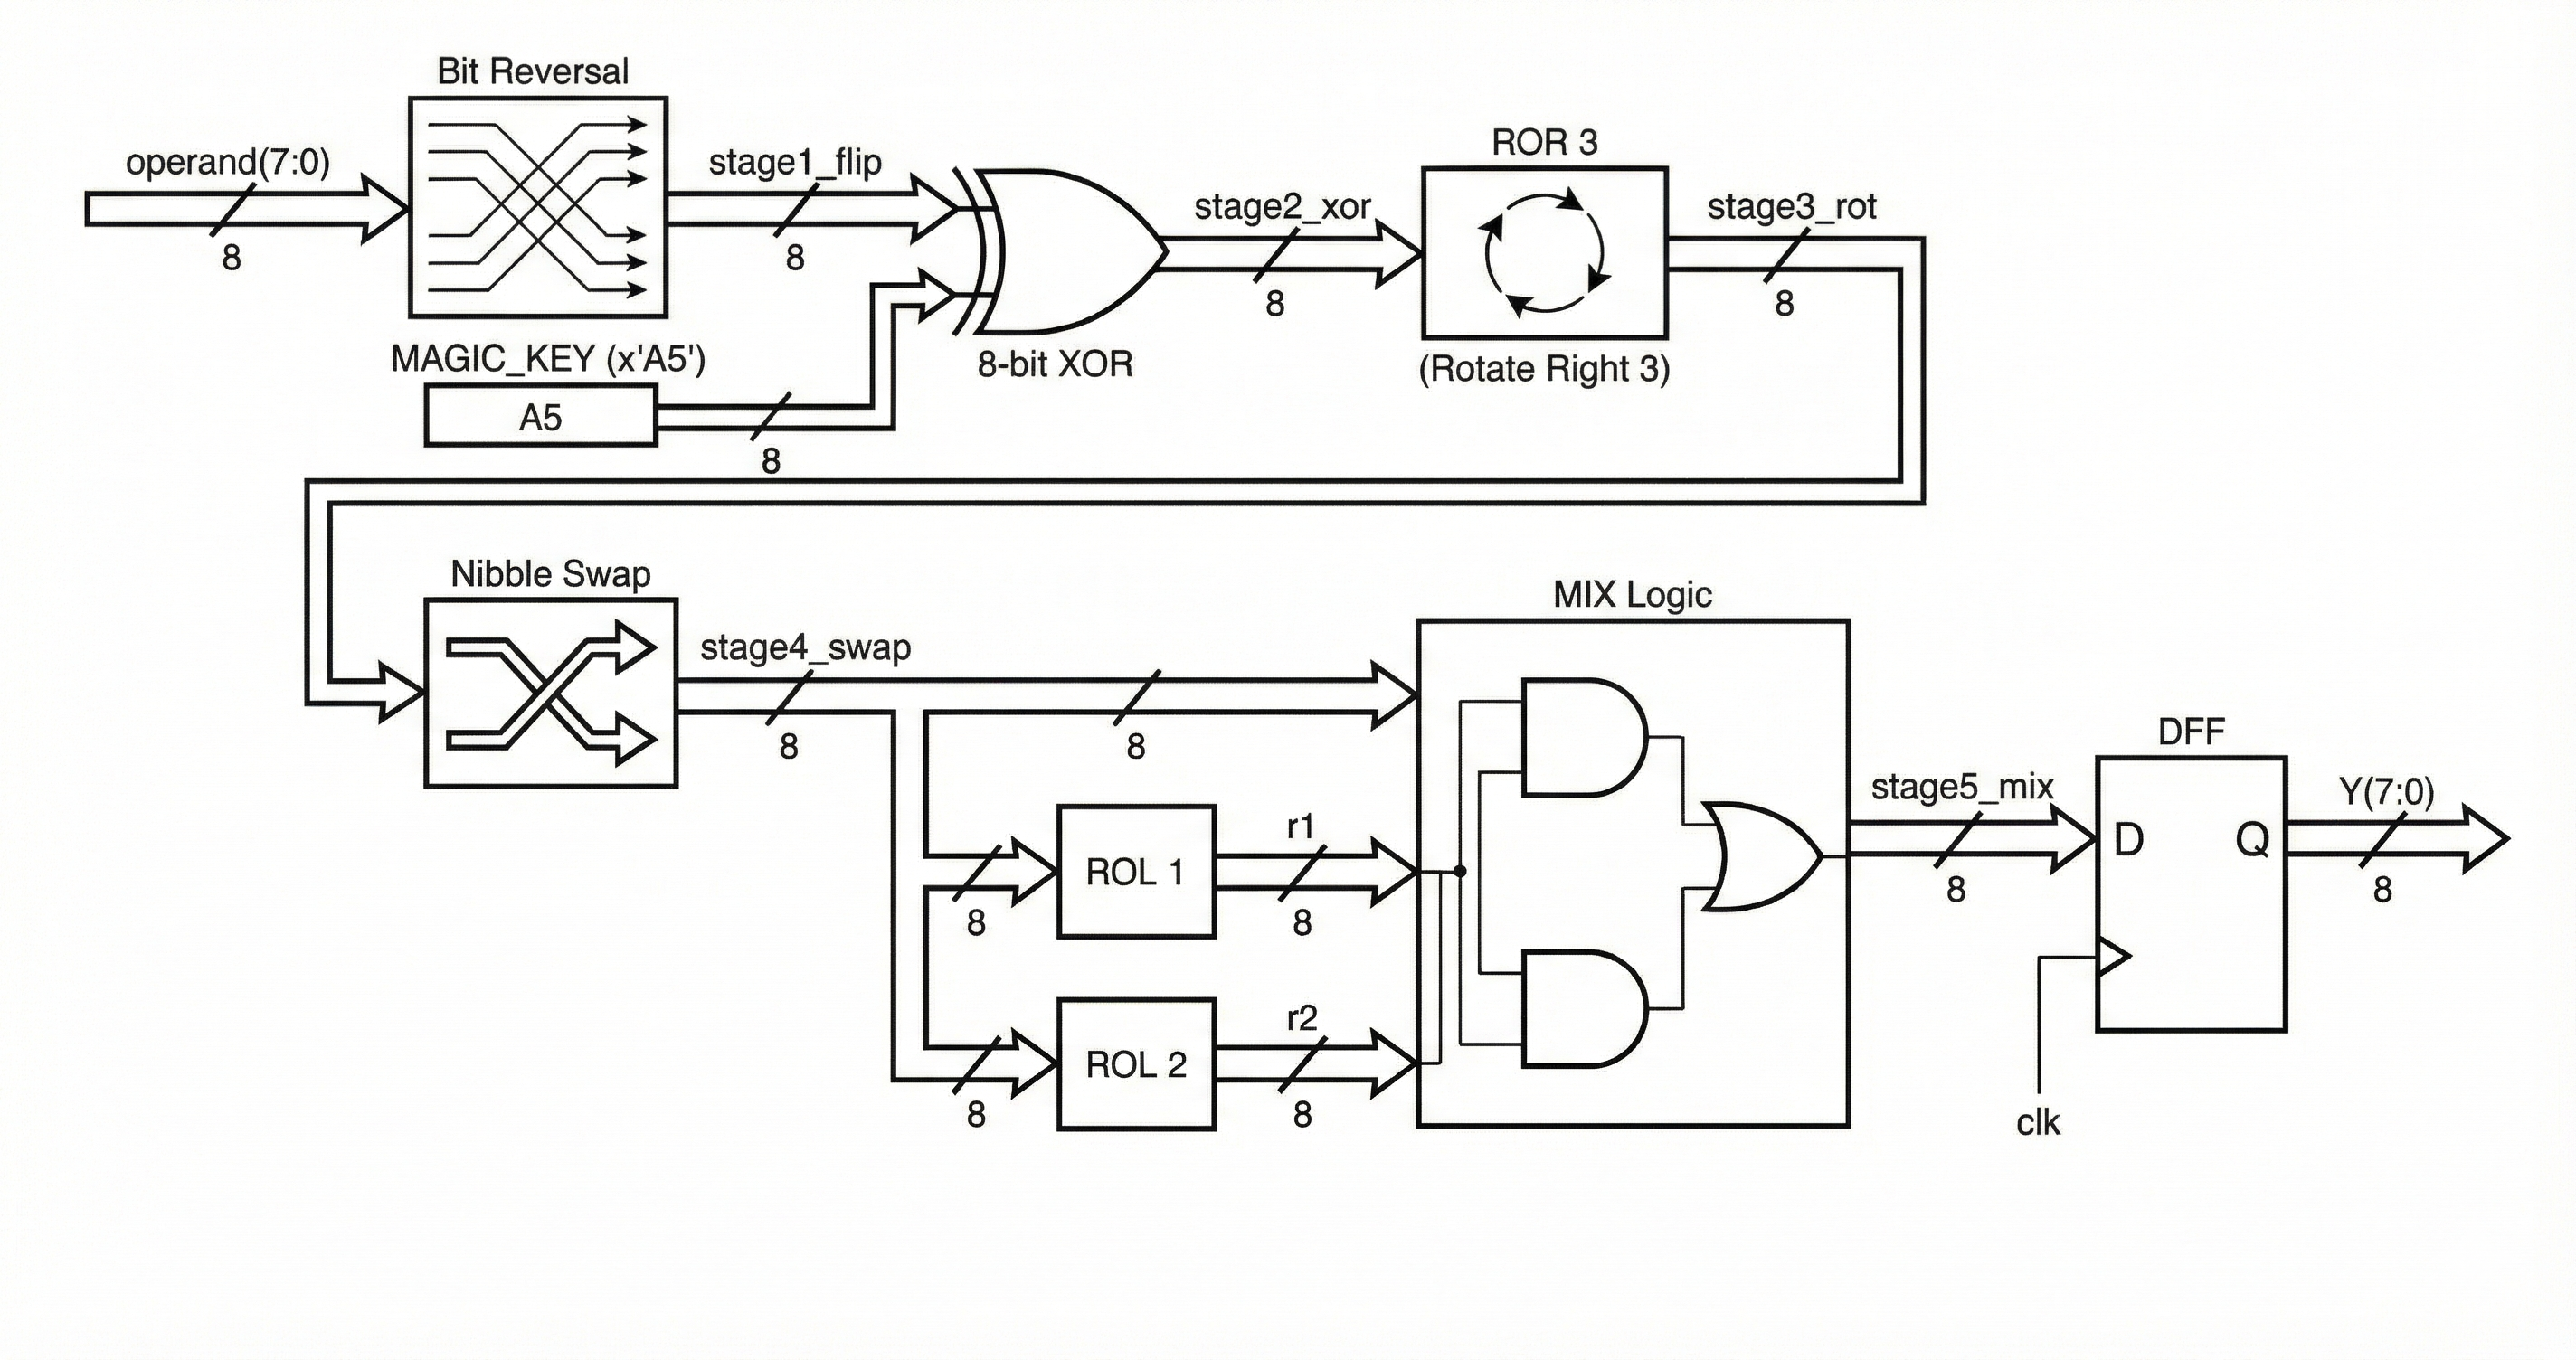
\includegraphics[width=0.9\textwidth]{resources/img/hasher.png}
 	\caption{Diagrama del módulo Hasher.}
 	\label{fig:hasher}
 \end{figure}


Como se muestra en la figura anterior, la arquitectura del módulo hasher se compone de 5 etapas en cascada:

\texttt{stage1\_flip:} La primera transformación invierte el orden de los bits del operando de entrada. Lo que tendríamos antes como flip. El bit 0 pasa a ser el bit 7, el bit 1 pasa a ser el bit 6, y así sucesivamente.

\begin{lstlisting}[language=VHDL, caption={Etapa FLIP}]
flip_gen: for i in 0 to 7 generate
    stage1_flip(i) <= operand(7-i);
end generate;
\end{lstlisting}

\texttt{stage2\_xor:} El resultado de la etapa anterior se combina mediante una operación XOR con una constante denominada \texttt{MAGIC\_KEY} cuyo valor es \texttt{0xA5} (10100101 en binario). La clave mágina es lo que normalmente se conoce como clave privada, aunque en este caso está pensado para dejarlo en el código sin cambiar, de forma que desde fuera no se podría revelar.

\begin{lstlisting}[language=VHDL, caption={Etapa XOR}]
constant MAGIC_KEY : std_logic_vector(7 downto 0) := x"A5";
stage2_xor <= stage1_flip xor MAGIC_KEY;
\end{lstlisting}

\texttt{stage3\_rot:} Se realiza una rotación hacia la izquierda de 3 posiciones. Los 3 bits más significativos pasan a ocupar las posiciones menos significativas.

\begin{lstlisting}[language=VHDL, caption={Etapa ROT}]
stage3_rot <= stage2_xor(4 downto 0) & stage2_xor(7 downto 5);
\end{lstlisting}

\texttt{stage4\_swap:} Se intercambian los nibbles (grupos de 4 bits) del byte. El nibble alto pasa a ser el bajo y viceversa.

\begin{lstlisting}[language=VHDL, caption={Etapa NIBBLE SWAP}]
stage4_swap <= stage3_rot(3 downto 0) & stage3_rot(7 downto 4);
\end{lstlisting}

\texttt{stage5\_mix: }La etapa final aplica una mezcla no lineal utilizando rotaciones adicionales y operaciones lógicas:

\begin{lstlisting}[language=VHDL, caption={Etapa MIX}]
r1 <= stage4_swap(6 downto 0) & stage4_swap(7);          -- rotl1
r2 <= stage4_swap(5 downto 0) & stage4_swap(7 downto 6); -- rotl2
stage5_mix <= stage4_swap xor r1 xor (stage4_swap and r2);
\end{lstlisting}

Esta etapa combina el resultado anterior con dos versiones rotadas de sí mismo (1 y 2 posiciones respectivamente), añadiendo no linealidad mediante la operación AND.

El resultado final se registra de forma síncrona en el flanco de subida del reloj, lo que añade un ciclo de latencia pero mejora el timing del diseño.

%%%%%%%%%%%%%%%%%%%%%%%%%%%%%%%%%%%%%%%%%%%%%%%%%%%%%%%%%%%%%%%%%%%%%%%%%%%%%%%
\chapter{Periféricos}
%%%%%%%%%%%%%%%%%%%%%%%%%%%%%%%%%%%%%%%%%%%%%%%%%%%%%%%%%%%%%%%%%%%%%%%%%%%%%%%

\section{Comparador Combinacional}

El módulo \texttt{modulo\_xor} implementa la comparación entre la contraseña introducida por el usuario (ya hasheada) y la contraseña correcta almacenada en el sistema.

La idea de elegir al comparador como un periférico separado es para mantener la modularidad del diseño. De esta forma, el comparador puede ser probado y verificado de forma independiente antes de integrarlo con el resto del sistema. Además, es agnóstico respecto a la fuente de datos, el algoritmo que se use en el hasher, o si la vga está activa o no, de forma que cualquier problema de funcionamiento en otras partes no interfiere con la comparación.

\subsection{Funcionamiento}


\begin{figure}[H]
 	\centering
 	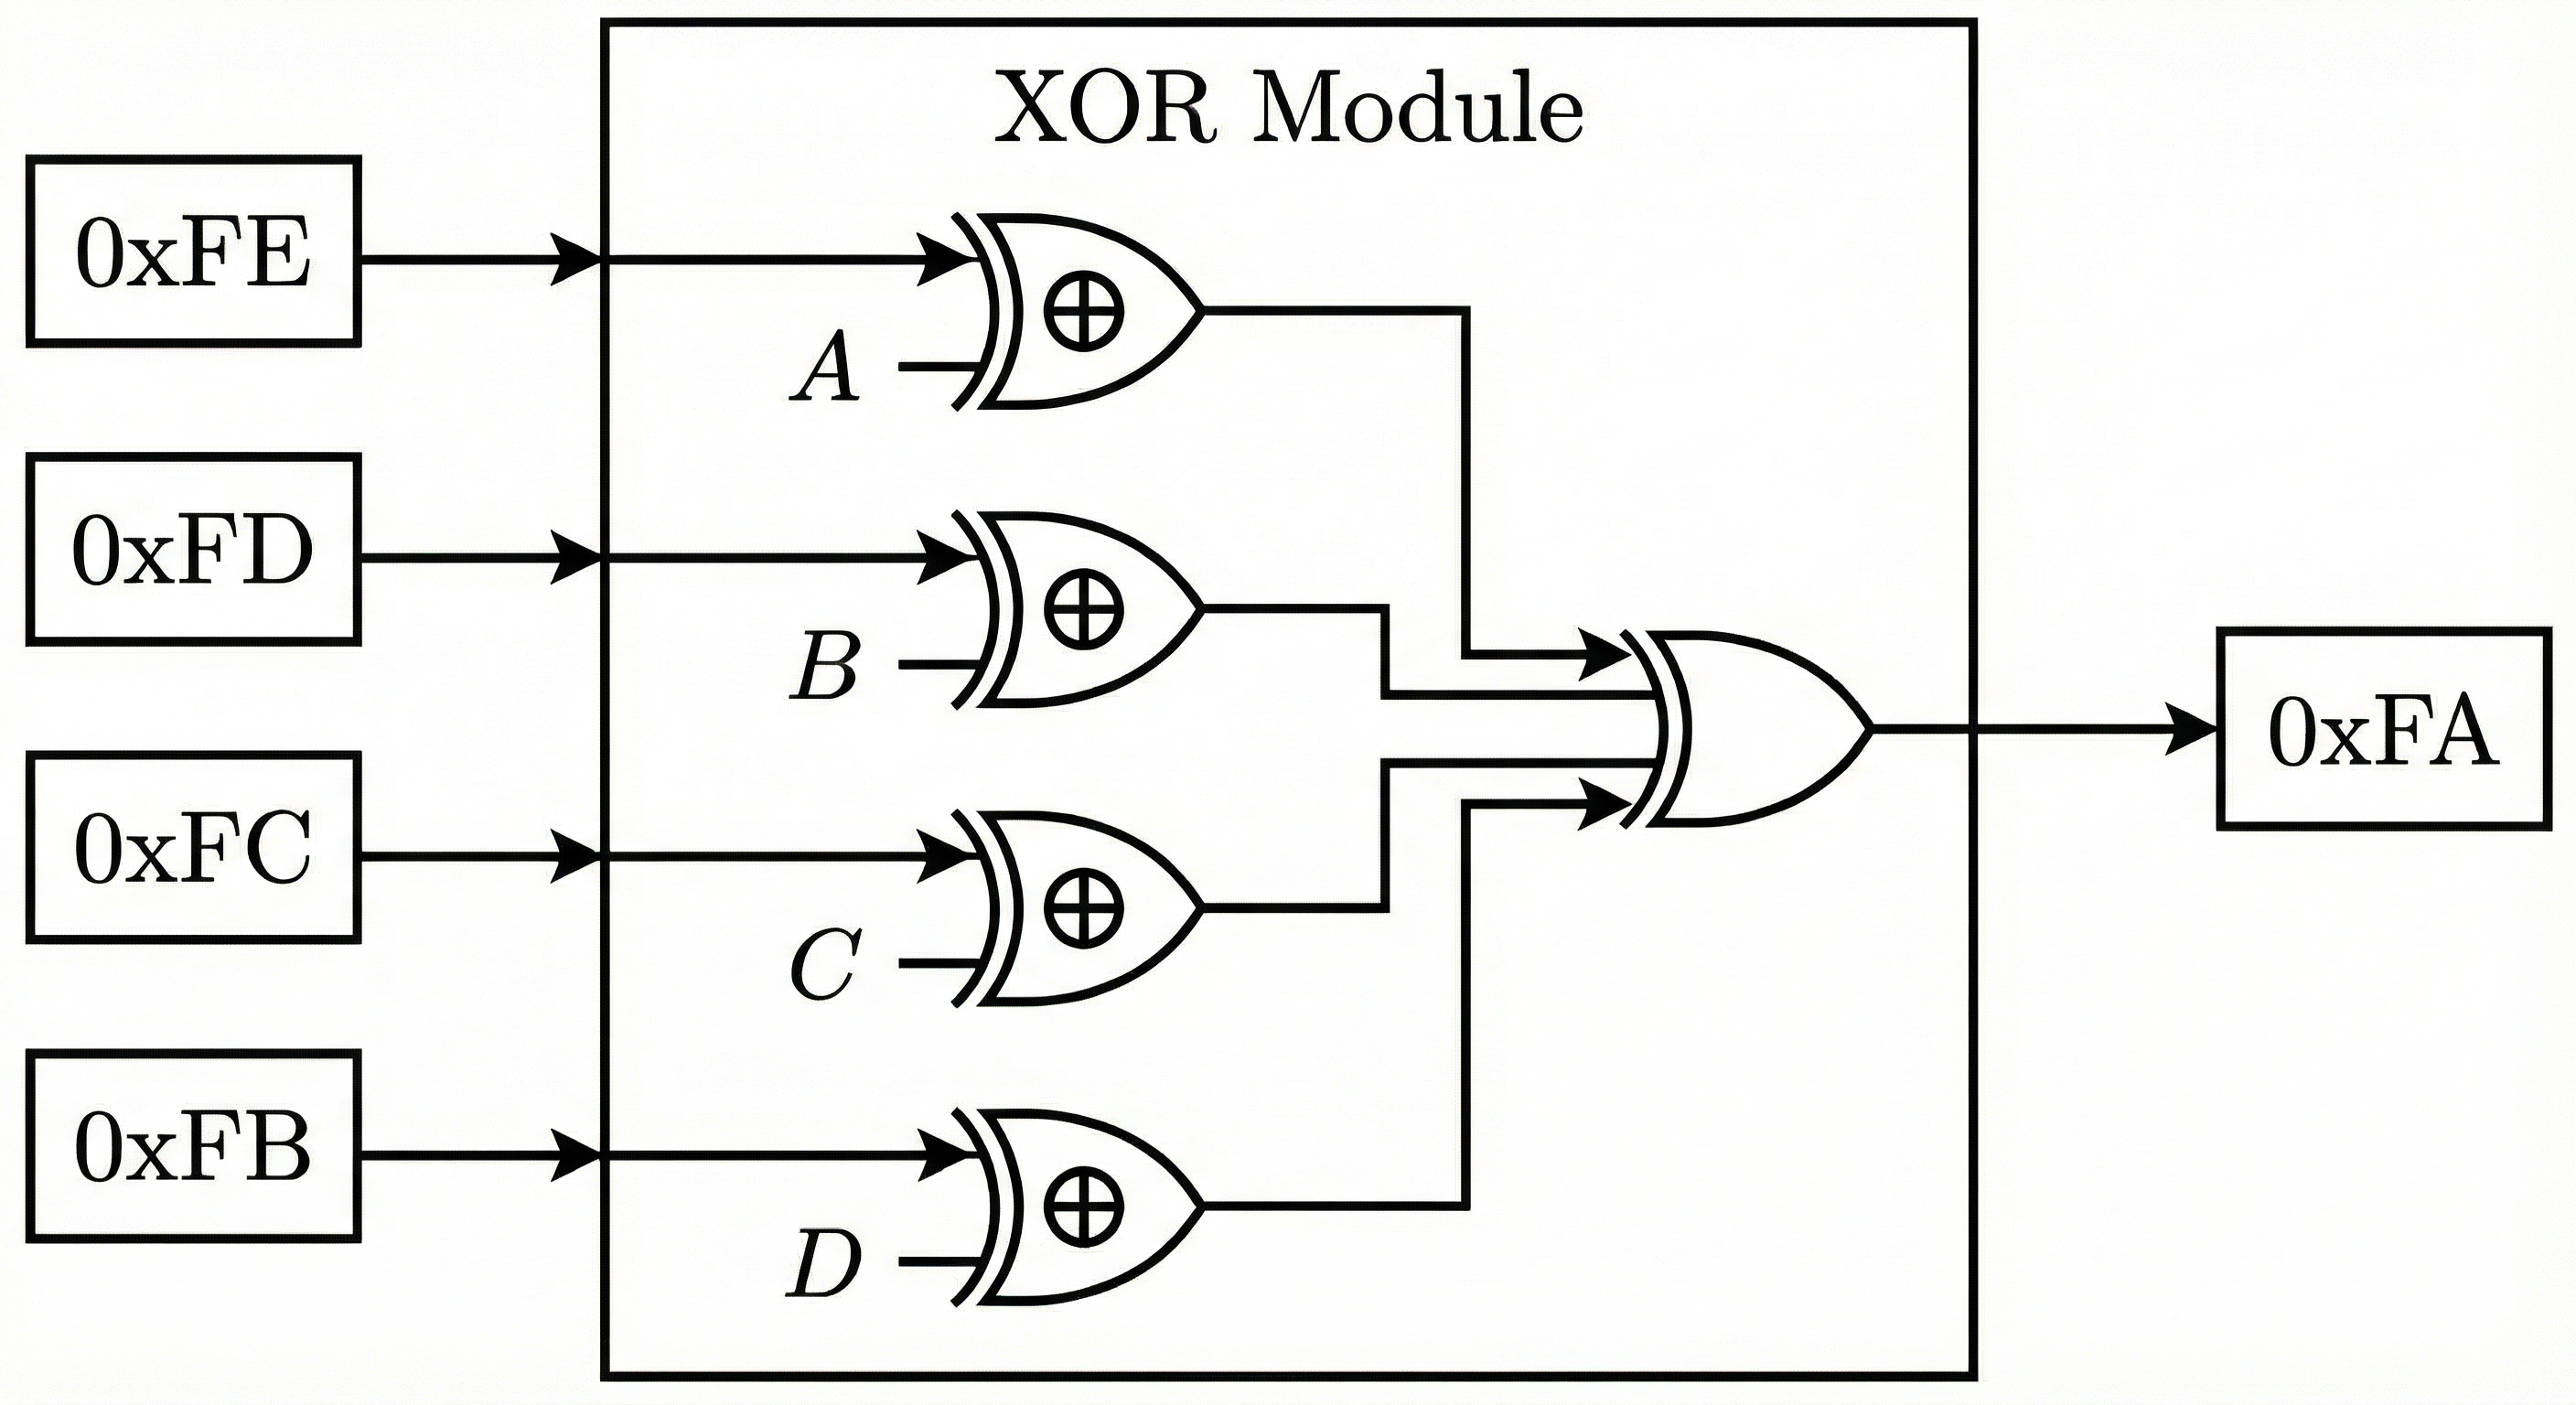
\includegraphics[width=0.7\textwidth]{resources/img/moduloxor.png}
 	\caption{Diagrama del comparador combinacional.}
 	\label{fig:moduloxor}
 \end{figure}

El módulo lee 4 caracteres hasheados a través de los puertos \texttt{0xFE}, \texttt{0xFD}, \texttt{0xFC} y \texttt{0xFB}. Estos valores se almacenan en registros internos cuando el PicoBlaze realiza una escritura (señal \texttt{write\_strobe} activa).

La contraseña correcta corresponde a la palabra ``HOLA'' procesada por el hasher:

\begin{lstlisting}[language=VHDL, caption={Contraseña hasheada almacenada}]
saved_char_1 <= "00101011";  -- 'H' hasheado
saved_char_2 <= "01011010";  -- 'O' hasheado
saved_char_3 <= "01011011";  -- 'L' hasheado
saved_char_4 <= "10110010";  -- 'A' hasheado
\end{lstlisting}

\subsection{Comparación}
La comparación se realiza mediante operaciones XOR entre cada carácter recibido y su correspondiente valor almacenado:

\begin{lstlisting}[language=VHDL, caption={Operaciones XOR de comparación}]
out_xor_1 <= saved_char_1 XOR char_1;
out_xor_2 <= saved_char_2 XOR char_2;
out_xor_3 <= saved_char_3 XOR char_3;
out_xor_4 <= saved_char_4 XOR char_4;
\end{lstlisting}

Si todos los resultados XOR son cero (es decir, todos los caracteres coinciden), el módulo devuelve \texttt{0x00} indicando éxito. En caso contrario, devuelve \texttt{0xFF} indicando fallo.

%%%%%%%%%%%%%%%%%%%%%%%%%%%%%%%%%%%%%%%%%%%%%%%%%%%%%%%%%%%%%%%%%%%%%%%%%%%%%%%
\section{VGA}

La interfaz VGA se implementa mediante dos módulos: \texttt{vga} (controlador base) y \texttt{vga\_inter} (interfaz con el sistema).

\subsection{Módulo VGA Base}

El módulo \texttt{vga} genera las señales de sincronización horizontal y vertical necesarias para una resolución de 640x480 píxeles a 60 Hz.

\subsubsection{Parámetros de temporización}
\begin{itemize}
    \item \textbf{Horizontal}: 794 píxeles totales por línea, con pulso de sincronía entre los píxeles 649 y 746.
    \item \textbf{Vertical}: 528 líneas totales por frame, con pulso de sincronía entre las líneas 489 y 491.
    \item \textbf{Área visible}: 640x480 píxeles (antes de los límites de inhibición).
\end{itemize}

El módulo utiliza un reloj de 25 MHz (habilitado mediante la señal \texttt{enable\_25Mhz}) para generar el timing correcto.

\subsection{Módulo VGA Inter}

El módulo \texttt{vga\_inter} actúa como interfaz entre el controlador VGA base y el sistema PicoBlaze. Su función principal es:

\begin{enumerate}
    \item Instanciar el módulo VGA base.
    \item Capturar el estado actual del sistema desde el bus del PicoBlaze (puerto \texttt{0xDD}).
    \item Generar el color de salida según el estado de la máquina de estados.
\end{enumerate}

\subsubsection{Codificación de colores}
\begin{itemize}
    \item \textbf{Estado de bloqueo con error} (\texttt{0x81}): Pantalla ROJA (\texttt{100}).
    \item \textbf{Estado de bloqueo acertado} (\texttt{0x82}): Pantalla VERDE (\texttt{010}).
    \item \textbf{Resto de estados}: Pantalla BLANCA (\texttt{111}).
\end{itemize}

%%%%%%%%%%%%%%%%%%%%%%%%%%%%%%%%%%%%%%%%%%%%%%%%%%%%%%%%%%%%%%%%%%%%%%%%%%%%%%%
\section{Máquina de Estados}

El módulo \texttt{estados} implementa una máquina de estados finita (FSM) que controla el flujo del sistema de autenticación.

\subsection{Estados definidos}

\begin{enumerate}
    \item \textbf{estado\_bloqueo}: Estado inicial y de penalización. El sistema permanece bloqueado durante 5 segundos (250 millones de ciclos a 50 MHz).
    \item \textbf{estado\_escucha}: El sistema está listo para recibir intentos de autenticación.
    \item \textbf{estado\_error1}: Primer intento fallido. Quedan 2 intentos.
    \item \textbf{estado\_error2}: Segundo intento fallido. Queda 1 intento.
    \item \textbf{estado\_error3}: Tercer intento fallido. Transición automática a bloqueo.
    \item \textbf{estado\_bien}: Autenticación exitosa. Transición automática a bloqueo.
\end{enumerate}

\subsection{Arquitectura de la FSM}

La máquina de estados sigue el patrón clásico de dos procesos:

\subsubsection{Proceso síncrono}
Gestiona la actualización del estado actual y el contador del temporizador. El contador solo avanza cuando el sistema está en estado de bloqueo.

\subsubsection{Proceso combinacional}
Determina el siguiente estado basándose en:
\begin{itemize}
    \item El estado actual.
    \item Las señales de comunicación del PicoBlaze (\texttt{write\_strobe}, \texttt{port\_id}).
    \item El valor recibido (\texttt{0x00} = acierto, \texttt{0xFF} = fallo).
    \item El valor del temporizador (para salir del bloqueo).
\end{itemize}

\subsection{Salidas}

El módulo genera una salida de 8 bits (\texttt{out\_result}) que codifica el estado actual:
\begin{itemize}
    \item \texttt{0x81}: Estado de bloqueo (bit 7 activo indica bloqueo al software).
    \item \texttt{0x01}: Estado de escucha.
    \item \texttt{0x02}: Error 1.
    \item \texttt{0x04}: Error 2.
\end{itemize}

Por lo que la estructura de la maquina de estados finita queda como:

\begin{figure}[H]
 	\centering
 	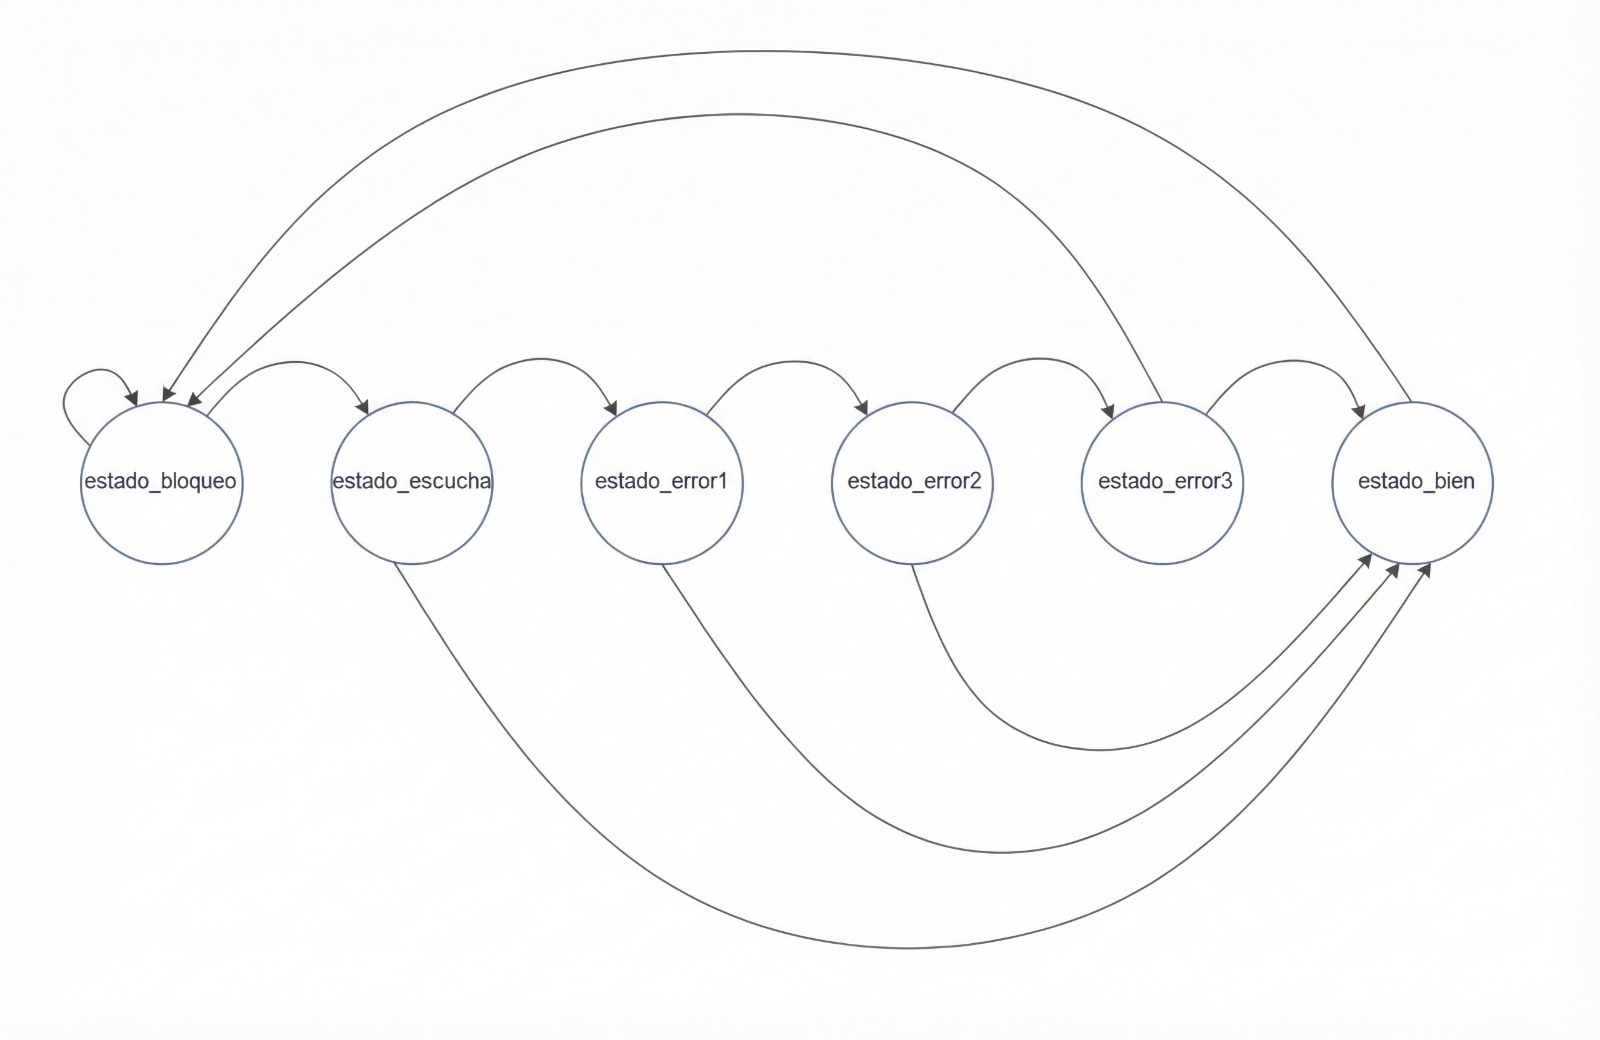
\includegraphics[width=0.7\textwidth]{resources/img/fsm.jpeg}
 	\caption{Diagrama del comparador combinacional.}
 	\label{fig:fsm}
 \end{figure}

%%%%%%%%%%%%%%%%%%%%%%%%%%%%%%%%%%%%%%%%%%%%%%%%%%%%%%%%%%%%%%%%%%%%%%%%%%%%%%%
\chapter{Assembly}
%%%%%%%%%%%%%%%%%%%%%%%%%%%%%%%%%%%%%%%%%%%%%%%%%%%%%%%%%%%%%%%%%%%%%%%%%%%%%%%


(POR MEJORAR)

El programa en ensamblador coordina todo el sistema, gestionando la comunicación serie, la interacción con los periféricos hardware y la presentación de resultados al usuario.

\section{Estructura del programa}



\subsection{Bucle principal}
El programa comienza verificando si el sistema está en estado de bloqueo consultando el puerto de la FSM. Si el bit 7 está activo, el programa espera en un bucle hasta que el bloqueo termine.

Una vez libre, el programa:
\begin{enumerate}
    \item Imprime un mensaje de bienvenida almacenado en RAM.
    \item Habilita las interrupciones.
    \item Entra en un bucle de espera, verificando continuamente el estado de bloqueo.
\end{enumerate}

\subsection{Rutina de interrupción}

Cuando el usuario envía un carácter por el puerto serie, se dispara la interrupción. La rutina:

\begin{enumerate}
    \item Deshabilita interrupciones para evitar reentrada.
    \item Verifica que no estemos en bloqueo.
    \item Recibe y hashea 4 caracteres consecutivos mediante la rutina \texttt{hashea}.
    \item Envía cada carácter hasheado al módulo comparador (puertos \texttt{0xFE}-\texttt{0xFB}).
    \item Lee el resultado de la comparación (puerto \texttt{0xFA}).
    \item Comunica el resultado a la FSM (puerto \texttt{0xDD}) y a la VGA (puerto \texttt{0xEF}).
    \item Muestra el mensaje correspondiente (``FELICIDADES'' o ``mal'').
    \item Retorna habilitando las interrupciones.
\end{enumerate}

\subsection{Rutina hashea}

Esta rutina encapsula el proceso de recibir un carácter, mostrar su eco por el puerto serie, y aplicar la instrucción \texttt{HASHER}:

\begin{lstlisting}[caption={Rutina hashea}]
hashea:
    CALL    recibe          ; Recibe caracter
    LOAD    txreg, rxreg    ; Copia para eco
    CALL    transmite       ; Envia eco
    HASHER  rxreg           ; Aplica hash
    RETURN
\end{lstlisting}

\subsection{Comunicación serie}

Las rutinas \texttt{recibe} y \texttt{transmite} implementan comunicación serie por software (bit-banging) a 9600 baudios. Utilizan temporizaciones precisas mediante las rutinas \texttt{wait\_1bit} y \texttt{wait\_05bit}.

%%%%%%%%%%%%%%%%%%%%%%%%%%%%%%%%%%%%%%%%%%%%%%%%%%%%%%%%%%%%%%%%%%%%%%%%%%%%%%%
\chapter{Extras}
%%%%%%%%%%%%%%%%%%%%%%%%%%%%%%%%%%%%%%%%%%%%%%%%%%%%%%%%%%%%%%%%%%%%%%%%%%%%%%%

aqui pongo la gilipollez del picowifi con la foto o un video o yo q se

%%%%%%%%%%%%%%%%%%%%%%%%%%%%%%%%%%%%%%%%%%%%%%%%%%%%%%%%%%%%%%%%%%%%%%%%%%%%%%%
\chapter{Conclusiones}
%%%%%%%%%%%%%%%%%%%%%%%%%%%%%%%%%%%%%%%%%%%%%%%%%%%%%%%%%%%%%%%%%%%%%%%%%%%%%%%

El desarrollo de este proyecto ha permitido explorar la integración de componentes hardware y software en un sistema embebido basado en PicoBlaze. Las principales conclusiones son:

\begin{enumerate}

    \item \textbf{Diseño modular}: La separación en módulos independientes (hasher, comparador, VGA, FSM) facilita el desarrollo, prueba y mantenimiento del sistema. Cada componente puede verificarse de forma aislada antes de la integración.

    \item \textbf{Interacción hardware-software}: El proyecto ilustra cómo el software (programa en ensamblador, aplicaciones externas como RS-232 o el picowifi) y el hardware (periféricos VHDL) cooperan para implementar funcionalidad compleja. El PicoBlaze actúa como coordinador mientras los periféricos realizan tareas especializadas.

    \item \textbf{Seguridad por diseño}: Aunque se trata de un sistema didáctico, incorpora principios básicos de seguridad como el hash de contraseñas, límite de intentos y tiempo de bloqueo. Esto demuestra cómo implementar mecanismos de seguridad a nivel hardware.

    \item \textbf{Retroalimentación visual}: La integración de la salida VGA proporciona una interfaz visual inmediata del estado del sistema, complementando la comunicación serie tradicional.
\end{enumerate}


\end{document}
